\documentclass{article}

\usepackage[utf8]{inputenc}
\usepackage[T1]{fontenc}
\usepackage[francais]{babel}
\usepackage{titling}
\setlength{\droptitle}{-3cm}
\usepackage{graphicx}
\usepackage{underscore}
\usepackage{hyperref} 


\title{Compte rendu : Jour 3}
\author{CAROT Axel, ARISOY Ivan Can, \\ BREILLAD Matis, BELKHITER Medhi}
\date{\today}

\begin{document}
\maketitle

\section{Travail effectué}

\subsection{Radar plot}

\begin{figure}[h]
    \centering
    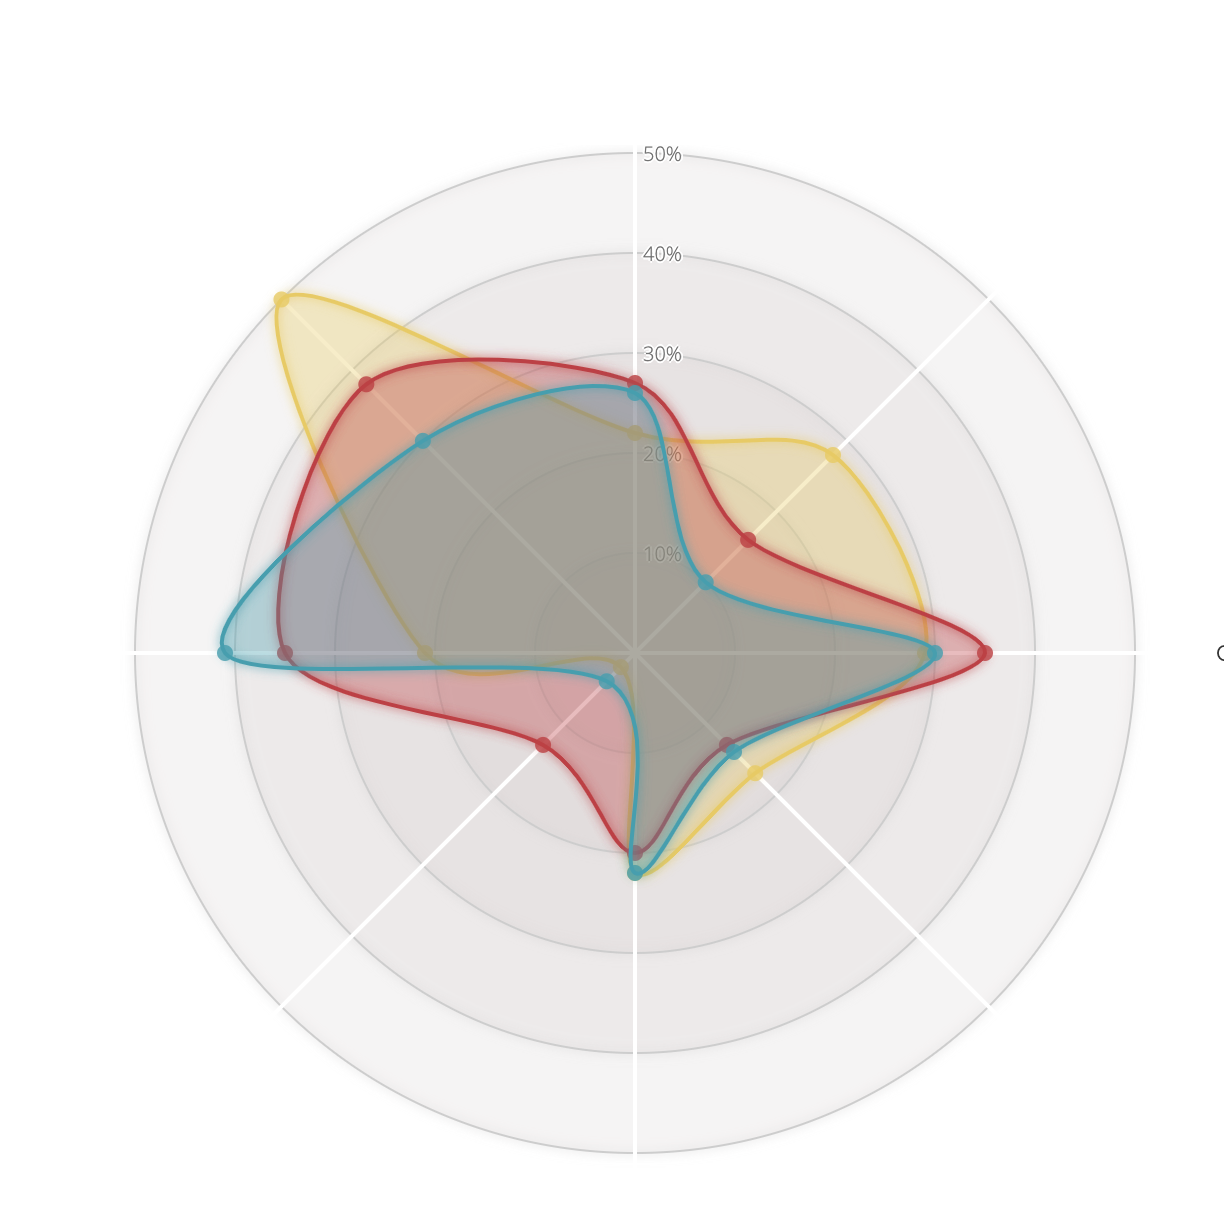
\includegraphics[width=0.3\textwidth]{radar.png}
    \caption{Radar plot}
    \label{fig:Radar plot}
\end{figure}

Nous avons commencé l'affichage du Radar plot avec D3js qui a posé de nombreux problèmes techniques. \\

Cette visualisation interactive permettra d'observer les valeurs des différentes variables concernant une communes choisit au préalable par l'utilisateur.

\subsection{Site}

\begin{figure}[h]
    \centering
    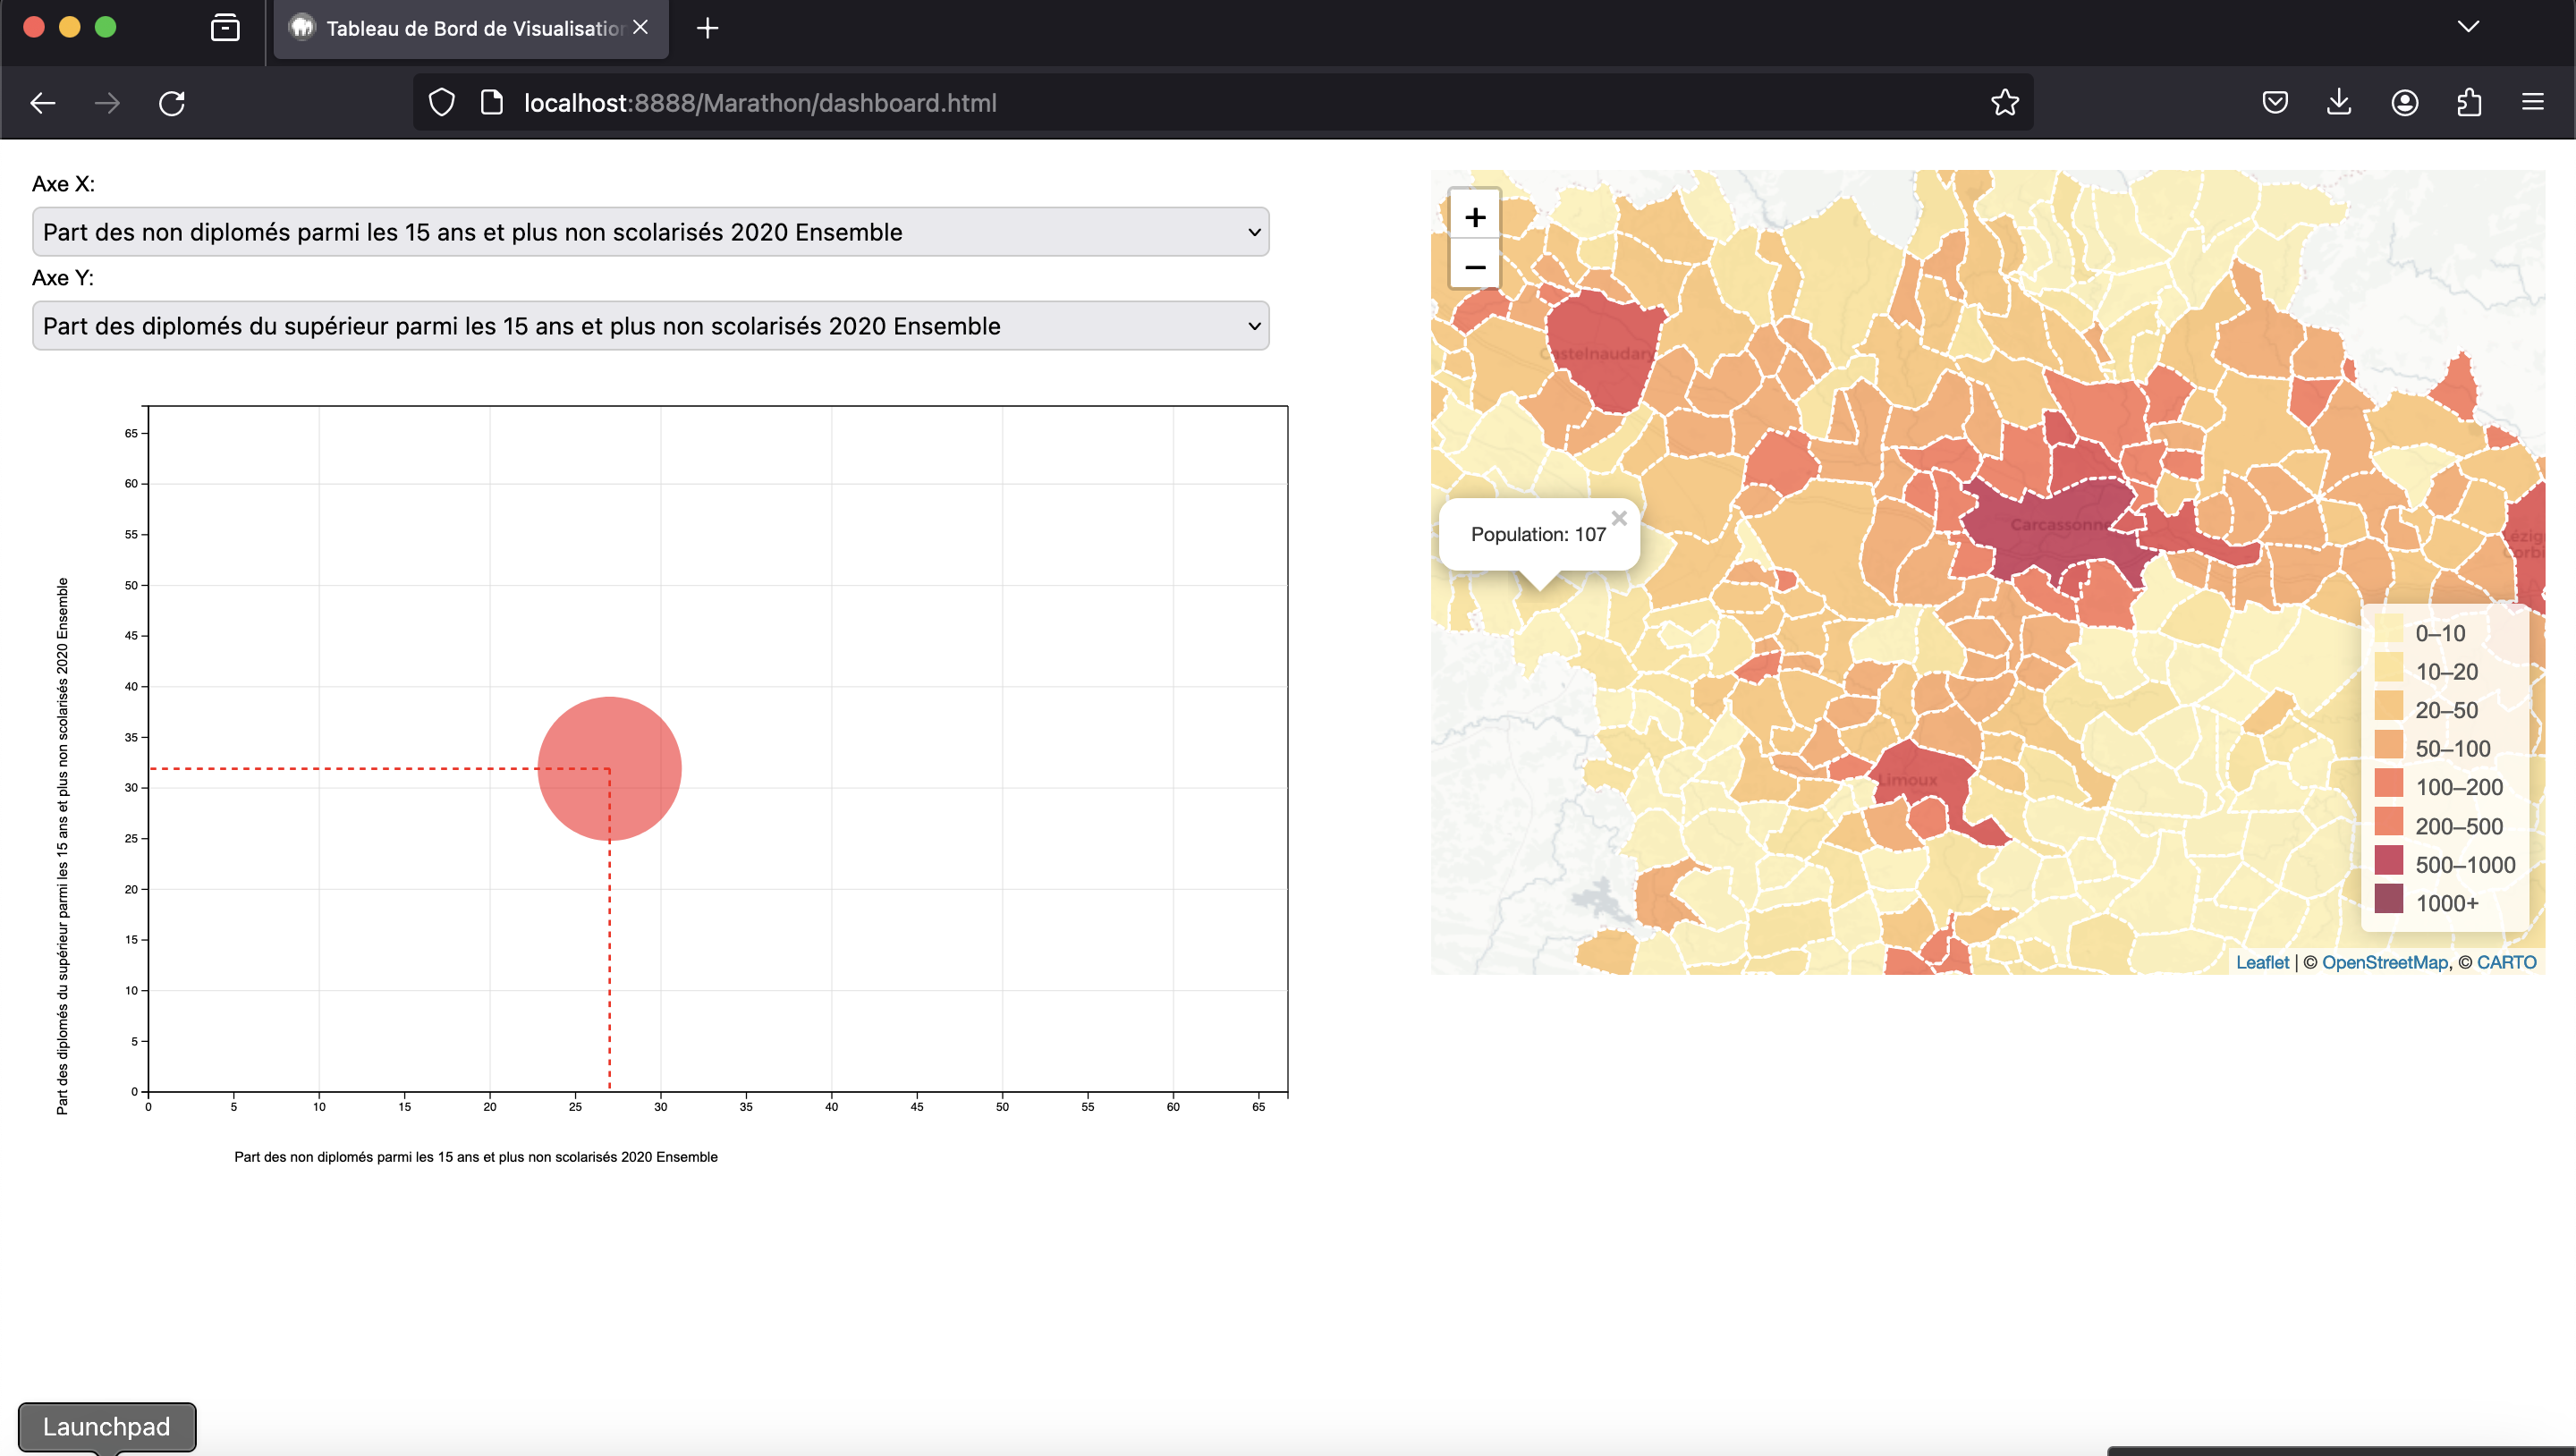
\includegraphics[width=0.7\textwidth]{medhi_site.png}
    \caption{Site}
    \label{fig:Site}
\end{figure}
\vspace{5cm}
Nous avons réussis à intégrer plusieurs visualisations faites avec D3 sur notre site. Nous avons aussi mis en place les liens entre les visualisations qui permettent que lorsqu'une commune est sélectionnée sur le graphique en bulle, elle soit aussi sélectionnée sur la carte. \\

\begin{figure}[h]
    \centering
    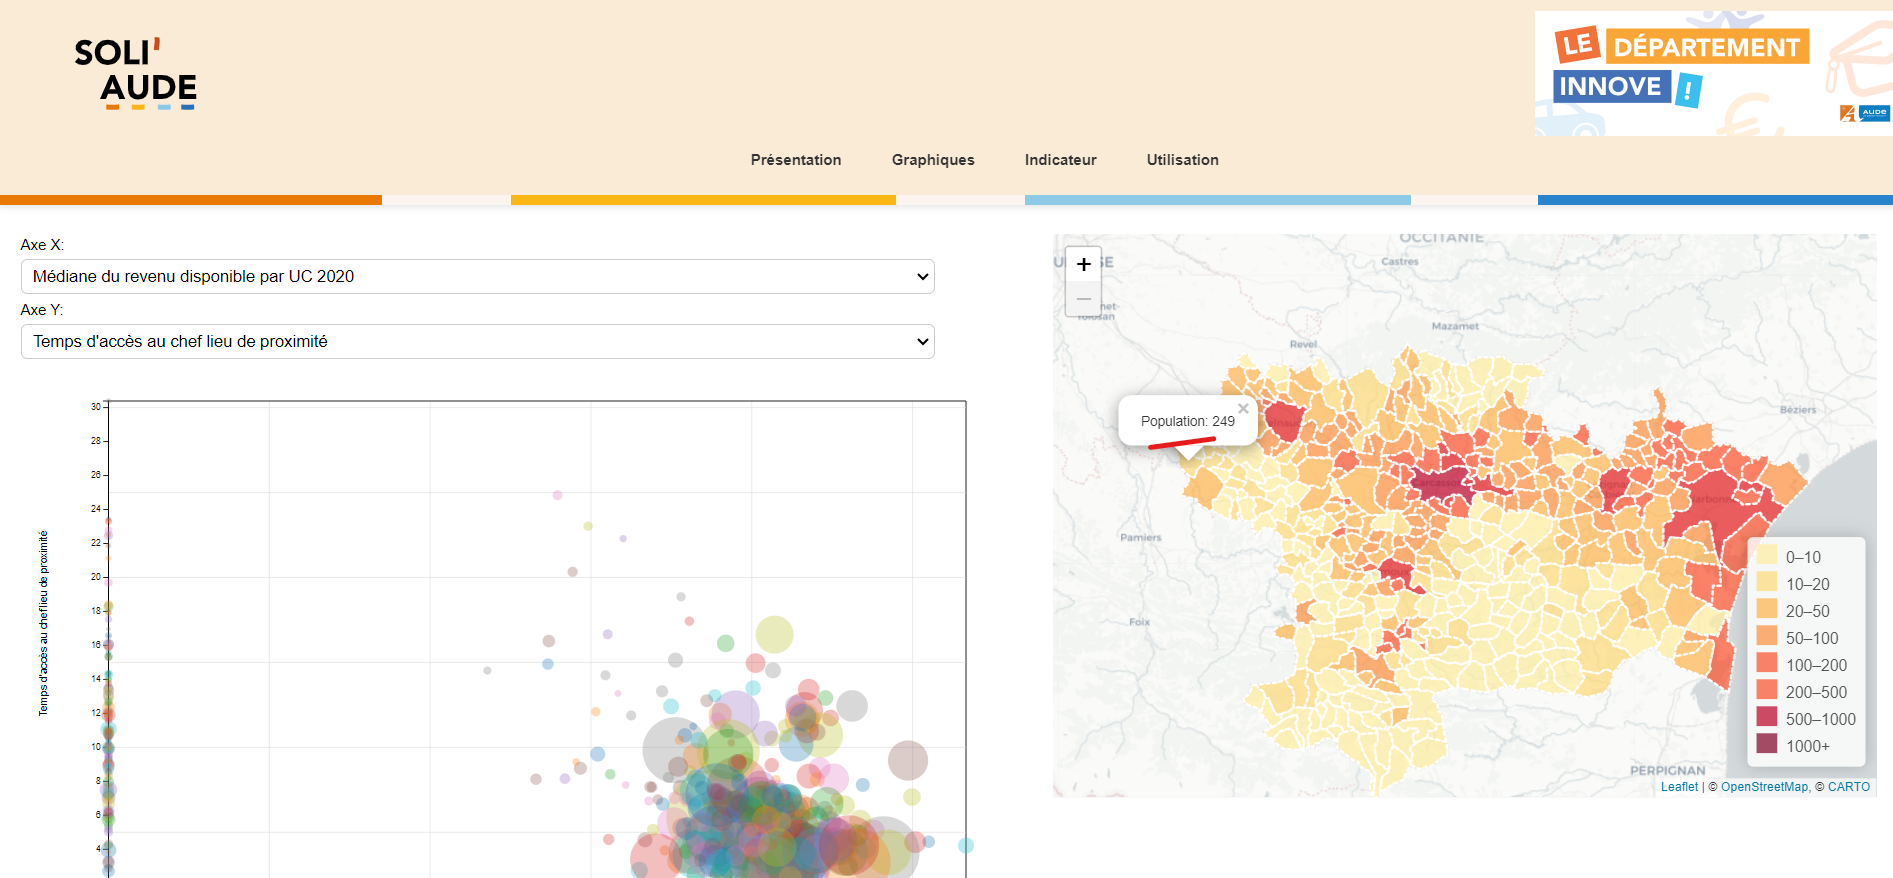
\includegraphics[width=1\textwidth]{mathis_site.png}
    \caption{Site}
    \label{fig:Site}
\end{figure}

Nous avons aussi commencé le design/front-end du site en essayant de respecter autant que possible la charte graphique mise en place par l'équipe du Master CNO (logo, couleurs ...) pour donner une identité visuelle cohérente au site et offrir une expérience utilisateur plus agréable.. Sur le screen les visualisations ne sont pas au niveau de nos avancés car nous essayons au maximum d'avancé en parallèle sur nos tâches respectives. 

\subsection{Indicateur}

Nous avons mis en place l'indicateur à l'aide des étapes suivantes : \\

\begin{itemize}
    \item Remplacement des données manquantes.
    \item Rescaling (min-max normalization) : consiste à mettre toutes les variables à la même échelle.
    \item Inversion d'échelle pour les colonnes avec une connotations négatives pour les communes (exemple : Taux de chômage des 15 ans et plus (RP) 2020).
    \item Ajout de la colonne Score qui est une moyenne pour chaque commune de toutes les valeurs la concernant dans les données. \\
\end{itemize} 

\begin{figure}[h]
    \centering
    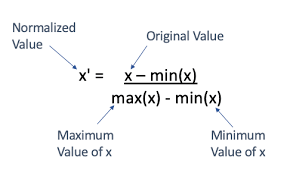
\includegraphics[width=0.5\textwidth]{normalisation.png}
    \caption{Rescaling (min-max normalization)}
    \label{fig:Rescaling (min-max normalization)}
\end{figure}
\vspace{2cm}
\section{Travail à faire}
\begin{itemize}
    \item Finaliser le radar plot avec D3.
    \item Développer l'affichage en D3 du calculateur utilisant l'indicateur.
    \item Réaliser un mode d'emploie de l'outil de Data viz.
    \item Continuer nos avancé sur le site qui regroupe les outils de visualisation et améliorer le front end du site.
\end{itemize} 

\end{document}
